To determine whether our \textbf{multi-modal} approach outperformed a traditional \textbf{vision only} approach to the language grounding problem in our \ispy task, we measured the average number of robot guesses and human guesses in games played with each fold of objects. Note that the systems were identical in fold 0, before receiving any training data.

\begin{figure}
\centering
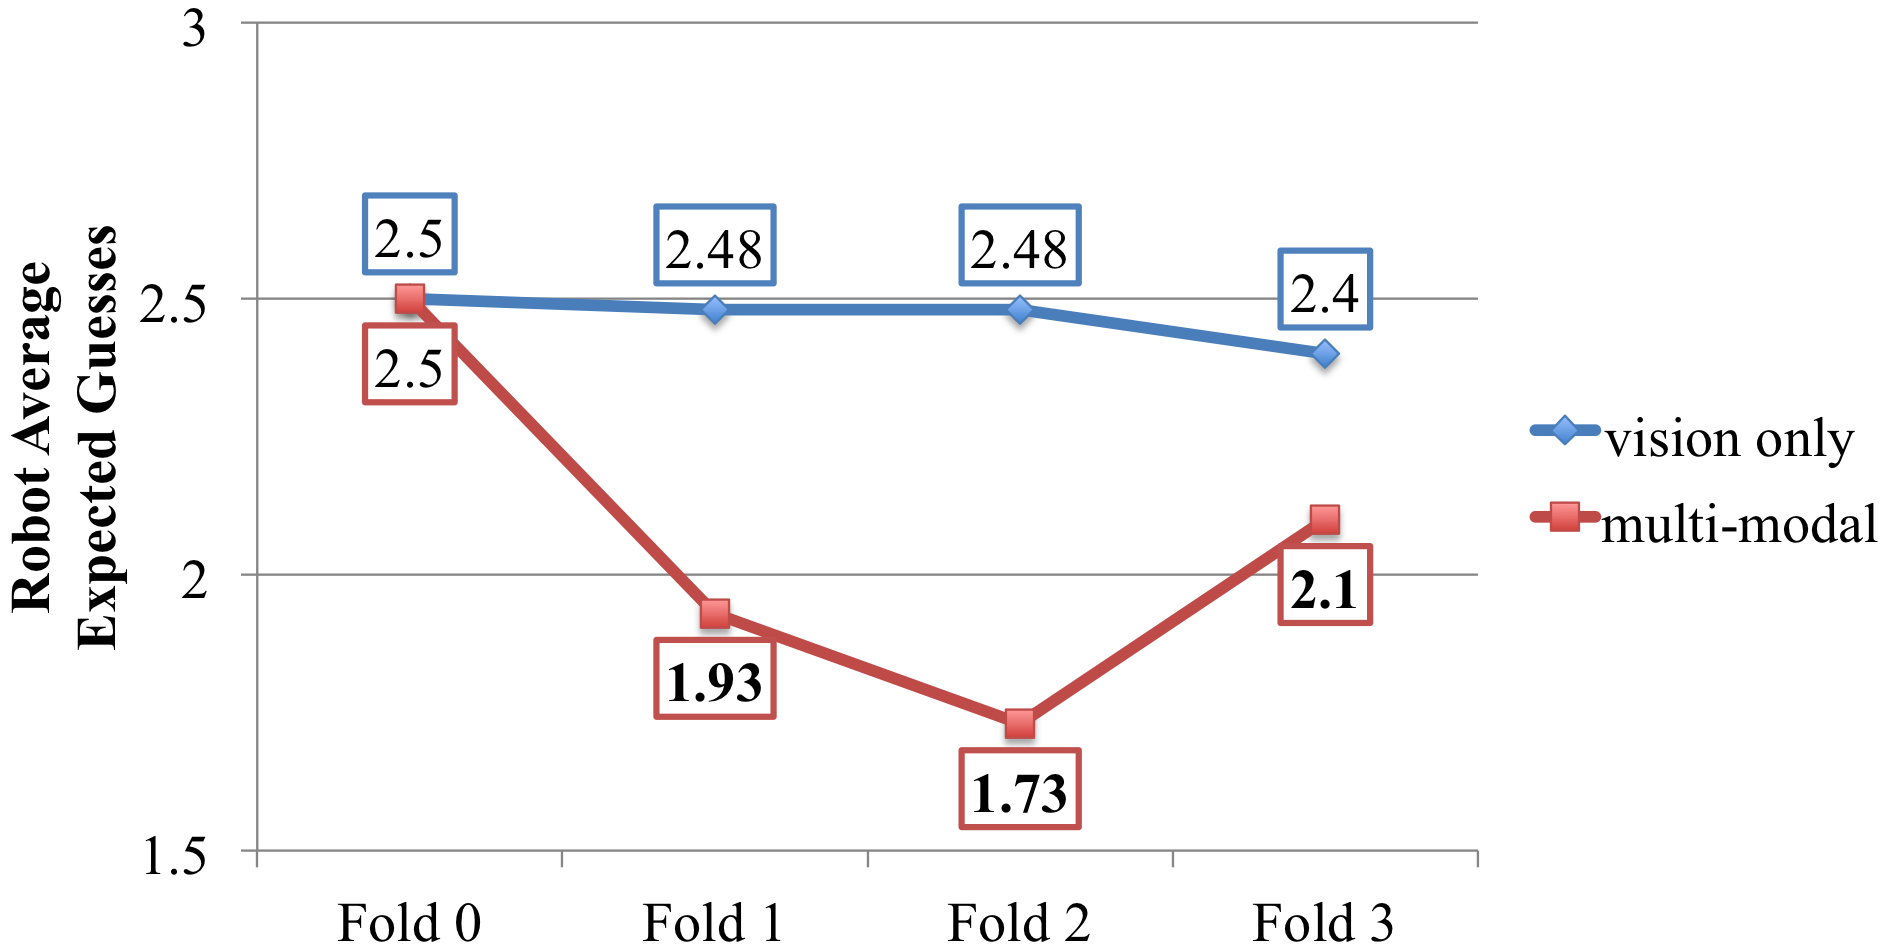
\includegraphics[width=0.5\textwidth]{figures/robot_guesses.png}
\caption{Average expected number of guesses the robot made on each human turn. Numbers in \textbf{bold} are significantly lower than the average at fold 0 with $p<0.05$ (unpaired Student's \textit{t}-test)}
\label{fig:robot_guesses}
\end{figure}

\paragraph{Robot guess.}
Figure~\ref{fig:robot_guesses} shows the average number of robot guesses across games in each fold. Because we had access to the order in which the robot intended to guess each object along with which objects were tied, we could calculate the expected number of guesses for each turn it took.
For example, if all four objects were tied for first to guess, we say the number of guesses for that turn was 2.5, regardless of whether it got (un)lucky and picked the correct object (last)first.

After training on just one fold, our \textbf{multi-modal} approach performs statistically significantly better than the expected number of turns for guessing (the only strategy for the untrained fold 0 system) for the remainder of the games.
The \textbf{vision only} system, by contrast, is never able to differentiate itself from a random guessing appraoch, even as more training data becomes available.
Additionally, on folds 1 and 2, a paired Student's \textit{t}-test ($p<0.05$) reveals that the \textbf{multi-modal} system outperms the \textbf{vision only} system on a subject-by-subject basis.
This difference could not be established for the more difficult fold 3 ($p=0.13$).

\begin{table}
\centering
\begin{tabular}{|l|r|r|r|r|}
	\hline
	\bf System & \multicolumn{4}{c|}{\bf Train Folds / Test Fold} \\ \hline \hline
	& \bf 123 / 0 & \bf 023 / 1 & \bf 013 / 2 & \bf 012 / 3 \\ \hline
	\bf vision only & 2.45 & 2.45 & 2.68 & 2.4 \\ \hline
	\bf multi-modal & 2.23 & 2.7 & 2.1 & 2.1 \\ \hline
\end{tabular}
\caption{Average expected number of robot guesses per cross-validated fold. For testing on folds other than 3, strictly less data was available at test time, yet no statistical differences in performance arose. Thus, the objects in fold 3 may be more difficult to learn properties of.}
\label{tab:crossval}
\end{table}

To explore the drop in performance we observe in fold 3, we cross-validated across the folds to simulate if the systems had been trained and tested on a different set of objects.
To make the evaluation fair, labels gained for words first seen in the new held-out fold by clarification questions on the robot's turn were discarded during training unless a user introduced them again in a description of an object.
This means these cross-validated systems each had strictly less training examples from which to learn.
Despite this, the average number of robot guesses for user descriptions in held-out folds was not statistically significantly different between any two (performances given in Table~\ref{tab:crossval}).
Given that the system performance on fold 3 is comparable to that on simulated, held-out folds for which there is strictly less training data, we argue that the objects in fold 3 may share fewer qualities with objects in other folds and are thus harder to learn about.

\begin{figure}
\centering
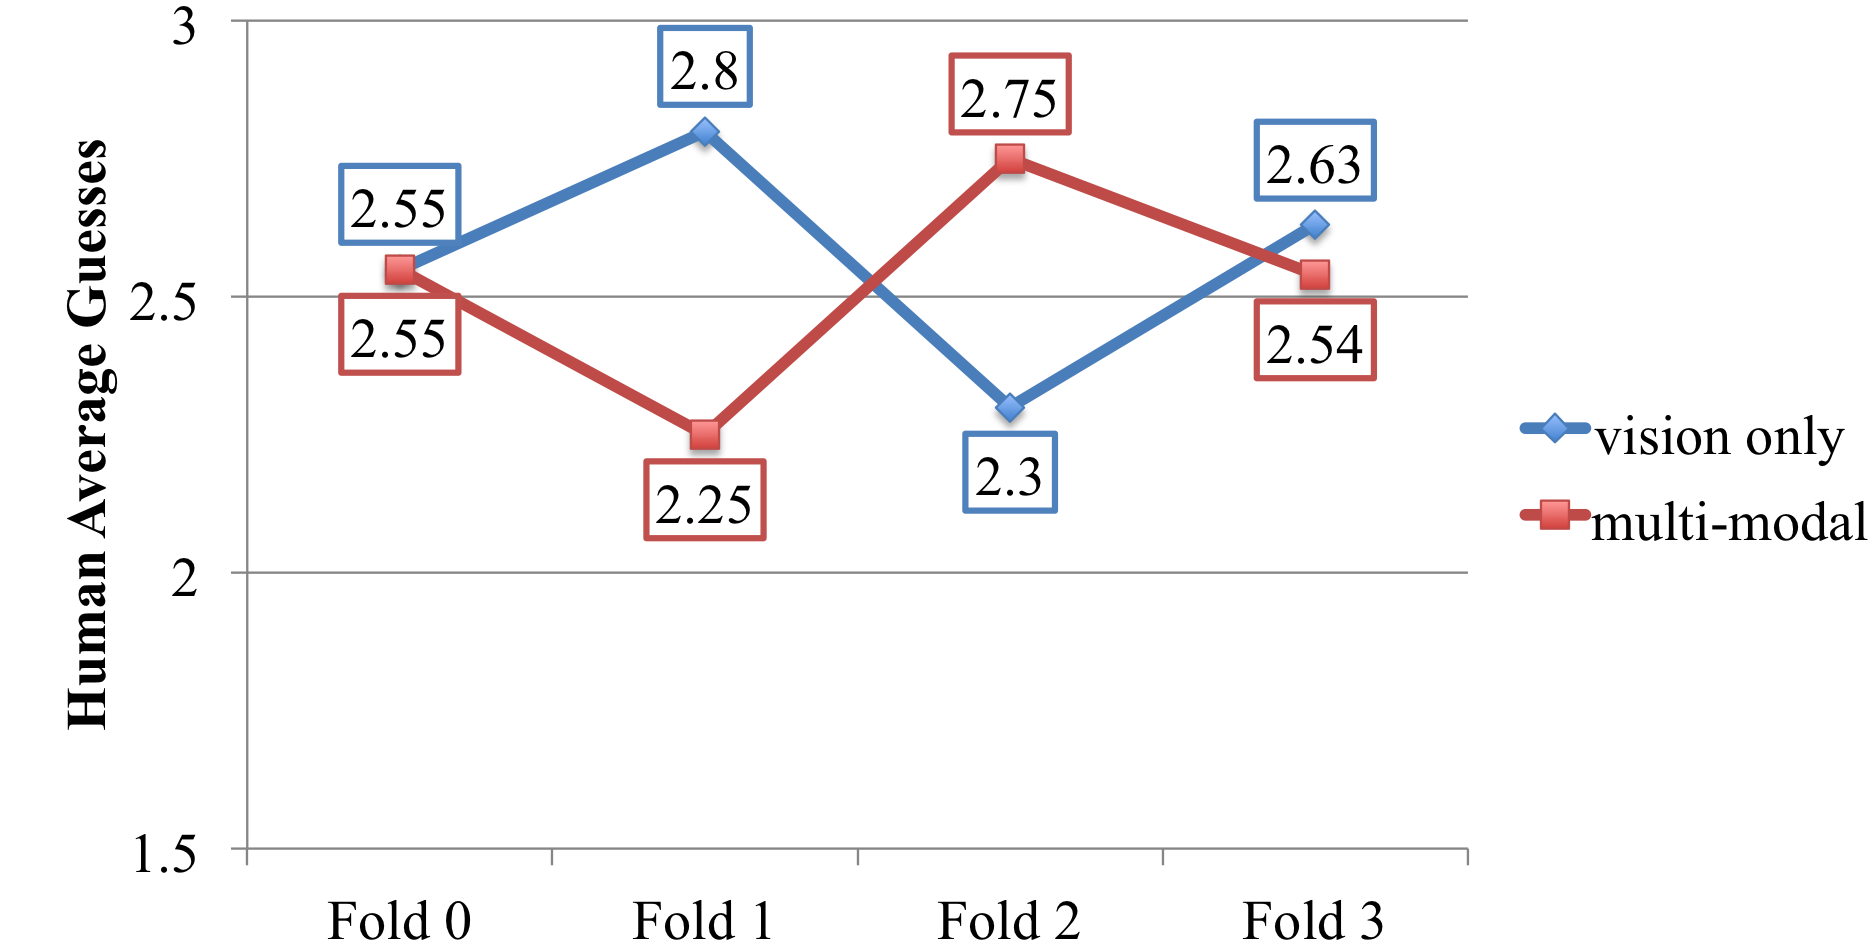
\includegraphics[width=0.5\textwidth]{figures/human_guesses.png}
\caption{Average expected number of guesses human subjects made on each robot turn.}
\label{fig:human_guesses}
\end{figure}

\paragraph{Human guess.}
Figure~\ref{fig:human_guesses} shows the average number of human guesses across games in each fold.
Since we have no such intuition into a human's guess order, we simply counted how many times a subject picked a new object as a guess.
We discarded guesses on the same object twice in a row, as these were often just double detections from the robot, but we counted guesses on the same object with an intervening guess after observing some users insisting to the robot that the object they had chosen before was correct.

Neither the \textbf{vision only} nor \textbf{multi-modal} system's performance appears to improve on this task as more training data becomes available.
In fact, Figure~\ref{fig:human_guesses} appears to show that human guesses hovered around 2.5 (random guessing) per robot turn throughout all levels of training and sets of objects.
Though our scoring system attempted to rank predicates highly if they both described an object well and differentiated it from the other options, it appears that subjects always effectively resorted to guessing.
This result highlights the difficulty of the robot's turn in an \ispy framework, and more generally of generating a salient description of an object for human understanding.